\section{CAP Theorem}
\begin{figure}[H]
    \centering
    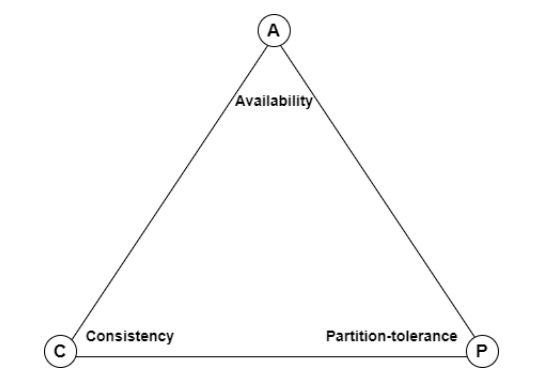
\includegraphics[scale=0.65]{cap.png}
    \caption{CAP Theorem}
    \label{fig::cap}
\end{figure}

CAP teorien er en database teori lavet af Eric Brewer i 1999, som bygger på at en database kan vælge mellem to af de tre punkter, som illustreret i figur XX. De tre punkter står for: 
\begin{itemize}
    \item C: Konsistent: Hver læsning modtager altid den seneste skrivning eller en fejl.
    \item A: Tilgængelighed: Hvert request modtager et validt svar, uden garanti for at det er den seneste skrivning.
    \item P: Partitionstolerance: Systemet fortsætter med at virke uanset om et vilkårligt antal af beskeder bliver forsinket eller forsvinder på netværket imellem noderne. 
\end{itemize}
Forskellige databasetyper går på kompromi med en af disse garantier. En database kan derfor enten være AC, AP eller CP. Hver har sine styrker og svagheder, som man skal tage i betragtning når man laver database design. CAP teorien bliver ofte refereret til sammen med ACID og BASE, som er databasemodeller der fundamentalt betegner hvordan en database håndtere begrænsningerne af CAP. Som eksempel på dette så er SQL databaser og de fleste NoSQL Graph databaser benytter sig af AC, som gør dem ACID kompatible, og dermed gør at de kan levere konsistens og tilgængelighed mellem noder i databasen. Dette er ikke muligt hvis der er partitioner, og gør at der ikke kan sikres fejltolerance som man får fra partitionstolerance. 